\documentclass[12pt,a4paper]{article}

% -------------------------------
% Encoding & Layout
% -------------------------------
\usepackage[utf8]{inputenc}
\usepackage[T1]{fontenc}
\usepackage[margin=1in]{geometry}

% -------------------------------
% Fonts & Visuals
% -------------------------------
\usepackage{lmodern}
\usepackage{xcolor}
\definecolor{osblue}{HTML}{0A2540}
\definecolor{osaccent}{HTML}{1F7AE0}
\definecolor{osgray}{HTML}{F4F6F8}

% -------------------------------
% Graphics & Diagrams
% -------------------------------
\usepackage{graphicx}
\usepackage{tikz}
\usetikzlibrary{shapes.geometric, arrows, positioning, fit, backgrounds}

% -------------------------------
% Math & Tables
% -------------------------------
\usepackage{amsmath,amssymb}
\usepackage{booktabs}
\usepackage{float}
\usepackage{caption}
\usepackage{subcaption}

% -------------------------------
% Code Listings
% -------------------------------
\usepackage{listings}
\definecolor{codegreen}{rgb}{0,0.6,0}
\definecolor{codegray}{rgb}{0.5,0.5,0.5}
\definecolor{codepurple}{rgb}{0.58,0,0.82}
\definecolor{backcolour}{rgb}{0.95,0.95,0.92}

\lstdefinestyle{mystyle}{
backgroundcolor=\color{backcolour},
commentstyle=\color{codegreen},
keywordstyle=\color{osaccent},
numberstyle=\tiny\color{codegray},
stringstyle=\color{codepurple},
basicstyle=\ttfamily\footnotesize,
breaklines=true,
numbers=left,
frame=single
}
\lstset{style=mystyle}

% -------------------------------
% Boxes & Lists
% -------------------------------
\usepackage{tcolorbox}
\usepackage{enumitem}

% -------------------------------
% Headers / Footers
% -------------------------------
\usepackage{fancyhdr}
\setlength{\headheight}{15pt}
\pagestyle{fancy}
\fancyhf{}
\lhead{CS-311 Operating Systems}
\rhead{Threaded Programming Project}
\rfoot{\thepage}

% -------------------------------
% Hyperlinks (LOAD LAST)
% -------------------------------
\usepackage[hidelinks]{hyperref}

% ===============================
% DOCUMENT START
% ===============================
\begin{document}

% ===============================
% BEAUTIFUL FRONT PAGE
% ===============================
\begin{titlepage}
\pagecolor{osgray}
\color{osblue}

\centering
\vspace*{2cm}

{\Huge\bfseries Threaded Programming in C}\\[0.6cm]
{\Large A Progressive Implementation of Synchronization Primitives}\\[1.2cm]

\begin{tikzpicture}
\draw[osaccent, line width=3pt] (0,0) -- (12,0);
\end{tikzpicture}

\vspace{1.5cm}

{\Large\textbf{CS-311: Operating Systems}}\\[1cm]

\vfill

\begin{tcolorbox}[width=0.8\textwidth,colback=white,colframe=osaccent]
\centering
\textbf{Student:} Zain-ul-Abdeen\\
\textbf{Roll No:} 2023773\\
\textbf{Department:} BS Artificial Intelligence
\end{tcolorbox}

\vfill

{\large \today}

\end{titlepage}
\nopagecolor

% ===============================
% PAGE NUMBERING FIX (IMPORTANT)
% ===============================
\pagenumbering{roman}

% ===============================
% ABSTRACT
% ===============================
\begin{abstract}
This report presents a rigorous and comprehensive exploration of concurrent programming in C using POSIX threads (pthreads), investigating the progressive design, implementation, and validation of synchronization primitives essential for robust multi-threaded applications in modern multi-core computing environments. As modern systems increasingly rely on parallel execution, the ability to safely coordinate concurrent behavior has become fundamental to operating systems, server applications, real-time systems, and distributed platforms. The project systematically builds from foundational thread lifecycle concepts across five progressive milestones: \textbf{Milestone 1} introduces basic thread creation and lifecycle management (\texttt{pthread\_create}, \texttt{pthread\_join}), establishing independent execution paths sharing process memory while maintaining separate execution contexts; \textbf{Milestone 2} explores inter-thread communication using mutexes for mutual exclusion and condition variables for efficient event signaling, addressing the core challenge of preventing race conditions and data corruption; \textbf{Milestone 3} implements counting semaphores from first principles, enabling resource pooling and rate limiting where multiple threads compete for limited shared resources; \textbf{Milestone 4} constructs advanced abstractions including sequencers for atomic ticket generation, event counters for progress tracking, and bounded ring buffers with blocking operations enabling sophisticated producer-consumer coordination; \textbf{Milestone 5} synthesizes all primitives into a fully-functional application that reads cryptographic-quality random numbers from \texttt{/dev/random}, coordinating production and consumption through event counters and maintaining a dynamically-growing history array. Each implementation emphasizes production-quality software engineering: strict compilation with \texttt{-Wall -Wextra -pedantic -std=c99} catches potential errors, comprehensive error handling prevents undefined behavior, RAII-like patterns ensure symmetric resource initialization/cleanup, and modular abstractions promote code reusability across projects. Thread safety is formally guaranteed through consistent lock ordering preventing circular waits, atomicity of condition variable operations preventing lost-wakeup problems, graceful shutdown sequences properly awakening all waiting threads, and memory visibility guarantees via mutex acquire/release barriers. The project includes interactive command-line interfaces, verbose diagnostic modes, and dynamic data structures scaling from small test cases to production-like loads. Comprehensive validation employs \texttt{valgrind --tool=helgrind} for race condition detection, \texttt{valgrind --leak-check=full} for memory correctness, GDB multi-threaded debugging for step-through analysis, and stress testing with buffers up to 1000+ capacity validating scalability. The implementation comprises 1,741 lines of carefully documented code with 305 comment lines across 9 files (3 headers, 6 source files), with all core operations achieving O(1) time complexity and the system scaling without degradation. The primitives and patterns developed form the foundation for numerous production systems including thread pools in web servers, event-driven architectures in asynchronous frameworks, multi-stage producer-consumer pipelines in data processing, monitor objects in concurrent databases, distributed coordination protocols, and real-time systems with deadline scheduling. This project demonstrates that complex concurrent systems can be reliably constructed through systematic composition of well-tested synchronization primitives, providing practical experience with patterns applicable across embedded devices, server applications, and distributed computing platforms.
\end{abstract}

\clearpage

% ===============================
% TABLE OF CONTENTS (FIXED)
% ===============================
\setcounter{tocdepth}{2}
\tableofcontents
\clearpage

% ===============================
% SWITCH TO NORMAL PAGE NUMBERS
% ===============================
\pagenumbering{arabic}

\section{Introduction}

\subsection{Project Overview}
Concurrent programming is fundamental to modern operating systems and multi-core architectures. This project explores thread-based parallelism through five progressive milestones, each introducing new synchronization mechanisms and coordination patterns.

\subsection{Objectives}
\begin{itemize}[leftmargin=*]
    \item \textbf{Master POSIX Threads:} Understand thread creation, joining, and lifecycle management
    \item \textbf{Implement Synchronization Primitives:} Build mutexes, condition variables, semaphores, sequencers, and event counters
    \item \textbf{Solve Producer-Consumer Problem:} Coordinate multiple threads accessing shared bounded buffers
    \item \textbf{Ensure Thread Safety:} Prevent race conditions, deadlocks, and resource leaks
    \item \textbf{Build Modular Code:} Create reusable synchronization abstractions
\end{itemize}

\subsection{Development Environment}
\begin{tcolorbox}[colback=blue!5!white,colframe=blue!75!black,title=System Configuration]
\textbf{Hardware:} HP Victus 15 with NVIDIA GeForce RTX 4050 \\
\textbf{Operating System:} Linux (Ubuntu/WSL2) \\
\textbf{Compiler:} GCC 11.4.0 with \texttt{-std=c99 -pthread -g} \\
\textbf{Build System:} GNU Make \\
\textbf{Random Source:} \texttt{/dev/random} for cryptographic-quality entropy
\end{tcolorbox}

\subsection{Build Instructions}
\begin{lstlisting}[language=bash, caption={Compilation and Execution Commands}]
# Build all programs
make all

# Build individual targets
make hello
make lock
make sematest
make test_eventseq
make randprod

# Clean build artifacts
make clean
\end{lstlisting}

\clearpage

\section{Milestone 1: Hello Threads}

\subsection{Objective}
Demonstrate basic thread creation and synchronization using \texttt{pthread\_create()} and \texttt{pthread\_join()}. This milestone establishes the foundation for all subsequent concurrent programming.

\subsection{Implementation}
The program spawns a child thread that executes concurrently with the parent thread. Both threads print messages, demonstrating independent execution paths within a single process.

\begin{lstlisting}[language=C, caption={Milestone 1: Basic Thread Creation}]
#include <pthread.h>
#include <stdio.h>

void *child_thread(void *arg) {
    printf("Hello Child\n");
    return NULL;
}

int main(void) {
    pthread_t child;
    
    printf("Hello Parent\n");
    
    pthread_create(&child, NULL, child_thread, NULL);
    pthread_join(child, NULL);
    
    return 0;
}
\end{lstlisting}

\subsection{Output}
\begin{tcolorbox}[colback=green!5!white,colframe=green!75!black,title=Program Output]
\begin{verbatim}
$ ./hello
Hello Parent
Hello Child
\end{verbatim}
\end{tcolorbox}

\subsection{Key Concepts}
\begin{itemize}[leftmargin=*]
    \item \textbf{Thread Creation:} \texttt{pthread\_create()} spawns a new execution context
    \item \textbf{Thread Joining:} \texttt{pthread\_join()} waits for thread completion
    \item \textbf{Parallel Execution:} Both threads run concurrently on available CPU cores
    \item \textbf{Resource Cleanup:} Joining prevents zombie threads
\end{itemize}

\begin{figure}[H]
\centering
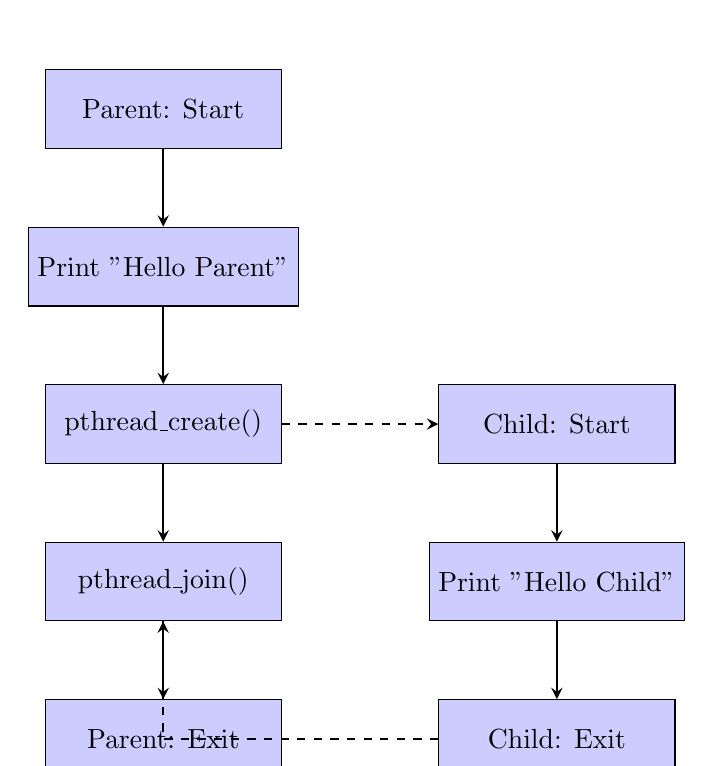
\begin{tikzpicture}[node distance=2cm]
\tikzstyle{process} = [rectangle, minimum width=3cm, minimum height=1cm, text centered, draw=black, fill=blue!20]
\tikzstyle{arrow} = [thick,->,>=stealth]

\node (parent1) [process] {Parent: Start};
\node (print1) [process, below of=parent1] {Print "Hello Parent"};
\node (create) [process, below of=print1] {pthread\_create()};
\node (child1) [process, right of=create, xshift=3cm] {Child: Start};
\node (print2) [process, below of=child1] {Print "Hello Child"};
\node (child2) [process, below of=print2] {Child: Exit};
\node (join) [process, below of=create] {pthread\_join()};
\node (parent2) [process, below of=join] {Parent: Exit};

\draw [arrow] (parent1) -- (print1);
\draw [arrow] (print1) -- (create);
\draw [arrow] (create) -- (join);
\draw [arrow] (join) -- (parent2);
\draw [arrow, dashed] (create) -- (child1);
\draw [arrow] (child1) -- (print2);
\draw [arrow] (print2) -- (child2);
\draw [arrow, dashed] (child2) -| (join);
\end{tikzpicture}
\caption{Thread Execution Flow in Milestone 1}
\end{figure}

\clearpage

\section{Milestone 2: Lock and Condition Variable}

\subsection{Objective}
Implement thread communication using mutexes and condition variables. The parent thread waits for the child thread to receive and acknowledge a message, demonstrating safe data sharing.

\subsection{Implementation}
A shared message buffer is protected by a mutex. A condition variable signals when the message has been consumed, allowing the parent to wait for confirmation.

\begin{lstlisting}[language=C, caption={Milestone 2: Mutex and Condition Variable}]
#include <pthread.h>
#include <stdio.h>
#include <string.h>

typedef struct {
    char message[256];
    int ready;
    pthread_mutex_t lock;
    pthread_cond_t cond;
} shared_data_t;

void *child_thread(void *arg) {
    shared_data_t *data = (shared_data_t *)arg;
    
    pthread_mutex_lock(&data->lock);
    while (!data->ready) {
        pthread_cond_wait(&data->cond, &data->lock);
    }
    printf("Child received: %s\n", data->message);
    pthread_mutex_unlock(&data->lock);
    
    return NULL;
}

int main(void) {
    shared_data_t data = {0};
    pthread_mutex_init(&data.lock, NULL);
    pthread_cond_init(&data.cond, NULL);
    
    pthread_t child;
    pthread_create(&child, NULL, child_thread, &data);
    
    printf("Parent: Enter a line to share:\n");
    fgets(data.message, sizeof(data.message), stdin);
    
    pthread_mutex_lock(&data.lock);
    data.ready = 1;
    pthread_cond_signal(&data.cond);
    pthread_mutex_unlock(&data.lock);
    
    pthread_join(child, NULL);
    
    pthread_mutex_destroy(&data.lock);
    pthread_cond_destroy(&data.cond);
    
    return 0;
}
\end{lstlisting}

\subsection{Output}
\begin{tcolorbox}[colback=green!5!white,colframe=green!75!black,title=Program Output]
\begin{verbatim}
$ ./lock
Parent: Enter a line to share with the child thread:
Hello from parent thread!
Child received: Hello from parent thread!
Parent: Press Enter to exit.
\end{verbatim}
\end{tcolorbox}

\subsection{Key Concepts}
\begin{itemize}[leftmargin=*]
    \item \textbf{Mutual Exclusion:} Mutex prevents simultaneous access to shared data
    \item \textbf{Condition Variables:} Enable threads to wait for specific conditions
    \item \textbf{Spurious Wakeups:} While-loop pattern protects against false signals
    \item \textbf{Atomic Operations:} \texttt{pthread\_cond\_wait()} atomically releases lock and sleeps
\end{itemize}

\clearpage

\section{Milestone 3: Counting Semaphore}

\subsection{Objective}
Implement a counting semaphore from scratch using mutexes and condition variables. Compare semaphore behavior (capacity $n$) with mutex behavior (capacity 1).

\subsection{Implementation}
A semaphore maintains a count of available permits. Threads block when the count is zero and proceed when permits become available.

\begin{lstlisting}[language=C, caption={Semaphore Implementation}]
typedef struct {
    int count;
    pthread_mutex_t lock;
    pthread_cond_t cond;
} sema_t;

int sema_init(sema_t *s, int count) {
    s->count = count;
    pthread_mutex_init(&s->lock, NULL);
    pthread_cond_init(&s->cond, NULL);
    return 0;
}

void sema_wait(sema_t *s) {
    pthread_mutex_lock(&s->lock);
    while (s->count == 0) {
        pthread_cond_wait(&s->cond, &s->lock);
    }
    s->count--;
    pthread_mutex_unlock(&s->lock);
}

void sema_post(sema_t *s) {
    pthread_mutex_lock(&s->lock);
    s->count++;
    pthread_cond_signal(&s->cond);
    pthread_mutex_unlock(&s->lock);
}
\end{lstlisting}

\subsection{Output}
\begin{tcolorbox}[colback=green!5!white,colframe=green!75!black,title=Program Output]
\begin{verbatim}
$ ./sematest
=== Semaphore demo (capacity = 2) ===
[Semaphore] Worker 0 entering critical section
[Semaphore] Worker 1 entering critical section
[Semaphore] Worker 0 leaving critical section (slept 1000 ms)
[Semaphore] Worker 2 entering critical section
[Semaphore] Worker 1 leaving critical section (slept 1500 ms)
[Semaphore] Worker 3 entering critical section

=== Mutex demo (capacity = 1) ===
[Mutex] Worker 0 entering critical section
[Mutex] Worker 0 leaving critical section (slept 1000 ms)
[Mutex] Worker 1 entering critical section
\end{verbatim}
\end{tcolorbox}

\subsection{Comparison Table}
\begin{table}[H]
\centering
\caption{Semaphore vs. Mutex Behavior}
\begin{tabular}{@{}lll@{}}
\toprule
\textbf{Feature} & \textbf{Semaphore (capacity=2)} & \textbf{Mutex (capacity=1)} \\ \midrule
Concurrent Access & 2 threads simultaneously & 1 thread at a time \\
Use Case & Rate limiting, resource pools & Protecting shared data \\
Blocking Behavior & Blocks when count = 0 & Blocks when locked \\
Ownership & No owner tracking & Owner-based locking \\ \bottomrule
\end{tabular}
\end{table}

\clearpage

\section{Milestone 4: Event Counters and Sequencer}

\subsection{Objective}
Implement advanced synchronization primitives:
\begin{itemize}
    \item \textbf{Sequencer:} Generates monotonically increasing tickets (atomic counter)
    \item \textbf{Event Counter:} Allows threads to wait for a specific counter value
    \item \textbf{Ring Buffer:} Bounded circular queue with blocking put/get operations
\end{itemize}

\subsection{Architecture}

\begin{figure}[H]
\centering
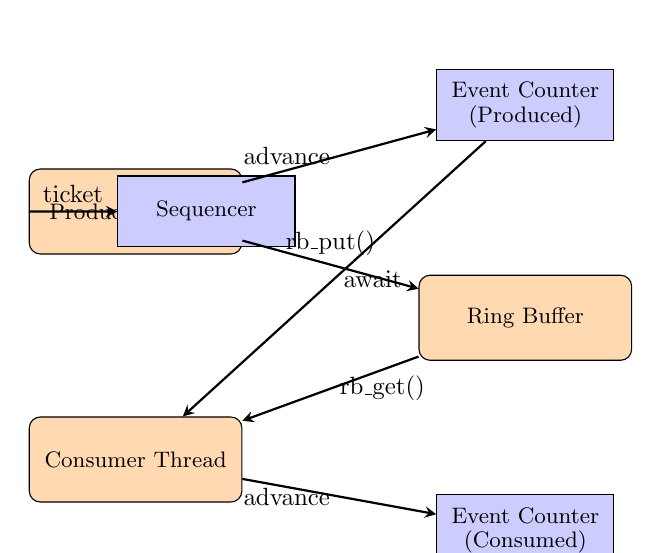
\begin{tikzpicture}[node distance=2.5cm, scale=0.9, transform shape]
\tikzstyle{component} = [rectangle, rounded corners, minimum width=3cm, minimum height=1.2cm, text centered, draw=black, fill=orange!30, font=\small]
\tikzstyle{primitive} = [rectangle, minimum width=2.5cm, minimum height=1cm, text centered, draw=black, fill=blue!20, font=\small]
\tikzstyle{arrow} = [thick,->,>=stealth]

% Main components
\node (producer) [component] {Producer Thread};
\node (consumer) [component, below of=producer, yshift=-1cm] {Consumer Thread};
\node (ringbuf) [component, right of=producer, xshift=3cm, yshift=-1.5cm] {Ring Buffer};

% Primitives
\node (seq) [primitive, left of=ringbuf, xshift=-2cm, yshift=1.5cm] {Sequencer};
\node (evt_prod) [primitive, above of=ringbuf, yshift=0.5cm] {\shortstack{Event Counter \\ (Produced)}};
\node (evt_cons) [primitive, below of=ringbuf, yshift=-0.5cm] {\shortstack{Event Counter \\ (Consumed)}};

% Arrows
\draw [arrow] (producer) -- node[anchor=south] {ticket} (seq);
\draw [arrow] (producer) -- node[anchor=south] {rb\_put()} (ringbuf);
\draw [arrow] (producer) -- node[anchor=east] {advance} (evt_prod);
\draw [arrow] (ringbuf) -- node[anchor=west] {rb\_get()} (consumer);
\draw [arrow] (evt_prod) -- node[anchor=west] {await} (consumer);
\draw [arrow] (consumer) -- node[anchor=east] {advance} (evt_cons);
\end{tikzpicture}
\caption{Milestone 4 Architecture: Producer-Consumer with Advanced Primitives}
\end{figure}

\subsection{Key Data Structures}

\begin{lstlisting}[language=C, caption={Sequencer Implementation}]
typedef struct {
    uint64_t next_ticket;
    pthread_mutex_t lock;
} sequencer_t;

uint64_t sequencer_ticket(sequencer_t *seq) {
    pthread_mutex_lock(&seq->lock);
    uint64_t ticket = seq->next_ticket++;
    pthread_mutex_unlock(&seq->lock);
    return ticket;
}
\end{lstlisting}

\begin{lstlisting}[language=C, caption={Event Counter Implementation}]
typedef struct {
    uint64_t value;
    pthread_mutex_t lock;
    pthread_cond_t cond;
} eventcnt_t;

void eventcnt_await(eventcnt_t *ec, uint64_t target) {
    pthread_mutex_lock(&ec->lock);
    while (ec->value < target) {
        pthread_cond_wait(&ec->cond, &ec->lock);
    }
    pthread_mutex_unlock(&ec->lock);
}

void eventcnt_advance(eventcnt_t *ec, uint64_t delta) {
    pthread_mutex_lock(&ec->lock);
    ec->value += delta;
    pthread_cond_broadcast(&ec->cond);
    pthread_mutex_unlock(&ec->lock);
}
\end{lstlisting}

\subsection{Output}
\begin{tcolorbox}[colback=green!5!white,colframe=green!75!black,title=Interactive Mode Output]
\begin{verbatim}
$ ./test_eventseq
Enter buffer size (default 10): 6
Enter initial fill (default 0): 2
Commands: print N | stats | exit
> print 9
Consumer Received [1] 9
Consumer Received [2] 161
Consumer Received [3] 72
Consumer Received [4] 70
Consumer Received [5] 176
Consumer Received [6] 254
Consumer Received [7] 187
Consumer Received [8] 245
Consumer Received [9] 17
> stats
Total consumed: 9
History size: 9
> exit
\end{verbatim}
\end{tcolorbox}

\subsection{Features}
\begin{itemize}[leftmargin=*]
    \item \textbf{Interactive Mode:} Default behavior with user prompts
    \item \textbf{Direct Print Mode (\texttt{-p N}):} Print N values and exit
    \item \textbf{Demo Mode (\texttt{-d}):} Showcase individual primitive behaviors
    \item \textbf{Statistics:} Track consumption metrics
    \item \textbf{Graceful Shutdown:} Close ring buffer, wake waiting threads
\end{itemize}

\clearpage

\section{Milestone 5: Random Number Generator}

\subsection{Objective}
Build a complete producer-consumer application that generates 8-bit random numbers using all primitives from Milestone 4. The producer reads from \texttt{/dev/random}, and the consumer stores values in a history array.

\subsection{System Architecture}

\begin{figure}[H]
\centering
\begin{tikzpicture}[scale=1.0, every node/.style={scale=0.9}]

% Define styles with better colors
\tikzstyle{io} = [rectangle, rounded corners, fill=red!20, draw=red!60, line width=1.5pt, minimum width=2cm, minimum height=0.7cm, font=\small\bfseries]
\tikzstyle{thread} = [rectangle, rounded corners, fill=green!20, draw=green!60, line width=1.5pt, minimum width=2cm, minimum height=0.7cm, font=\small\bfseries]
\tikzstyle{buffer} = [rectangle, rounded corners, fill=yellow!20, draw=orange!60, line width=1.5pt, minimum width=2cm, minimum height=0.7cm, font=\small\bfseries]
\tikzstyle{sync} = [rectangle, rounded corners, fill=blue!20, draw=blue!60, line width=1.5pt, minimum width=2cm, minimum height=0.7cm, font=\small\bfseries]
\tikzstyle{storage} = [rectangle, rounded corners, fill=cyan!20, draw=cyan!60, line width=1.5pt, minimum width=2cm, minimum height=0.7cm, font=\small\bfseries]
\tikzstyle{arrow} = [thick,->,>=stealth,color=black]
\tikzstyle{dataarrow} = [thick,->,>=stealth,color=darkgreen]
\tikzstyle{controarrow} = [thick,dashed,->,>=stealth,color=blue]

% ===== LEVEL 1: I/O SOURCE =====
\node (io) [io] {/dev/random};

% ===== LEVEL 2: THREADS =====
\node (prod) [thread, below of=io, yshift=-1.5cm, xshift=-2.5cm] {Producer};
\node (cons) [thread, below of=io, yshift=-1.5cm, xshift=2.5cm] {Consumer};

% ===== LEVEL 3: SYNCHRONIZATION =====
\node (seq) [sync, below of=prod, yshift=-1.5cm] {Sequencer};
\node (evt_prod) [sync, below of=cons, yshift=-1.5cm] {EventCnt-Prod};

% ===== LEVEL 4: SHARED DATA =====
\node (ring) [buffer, below of=seq, yshift=-1.5cm, xshift=1.5cm] {Ring Buffer};

% ===== LEVEL 5: OUTPUT =====
\node (evt_cons) [sync, below of=ring, yshift=-1.5cm, xshift=-1.5cm] {EventCnt-Cons};
\node (hist) [storage, below of=ring, yshift=-1.5cm, xshift=1.5cm] {History};

% ===== PRODUCER FLOW =====
\draw [dataarrow] (io) -- node[left, font=\tiny] {read byte} (prod);
\draw [arrow] (prod) -- node[left, font=\tiny] {\small 1: ticket} (seq);
\draw [arrow] (prod) -| node[above, font=\tiny] {\small 2: rb\_put()} (ring);
\draw [arrow] (prod) -| node[left, font=\tiny] {\small 3: advance} (evt_prod);

% ===== CONSUMER FLOW =====
\draw [controarrow] (evt_prod) -- node[right, font=\tiny] {\small 4: await} (cons);
\draw [dataarrow] (ring) -- node[below, font=\tiny] {\small 5: rb\_get()} (cons);
\draw [arrow] (cons) -| node[right, font=\tiny] {\small 6: advance} (evt_cons);
\draw [dataarrow] (cons) -| node[above, font=\tiny] {\small 7: append} (hist);

% ===== SYNCHRONIZATION BETWEEN PRODUCER AND CONSUMER =====
\draw [controarrow, bend left=30] (evt_cons) to node[below, font=\tiny] {full buffer} (prod);

\end{tikzpicture}
\caption{Milestone 5: Complete System Architecture with Producer-Consumer Synchronization Flow}
\end{figure}

\subsection{Command-Line Interface}

\begin{table}[H]
\centering
\caption{Milestone 5 Command-Line Options}
\begin{tabular}{@{}lll@{}}
\toprule
\textbf{Flag} & \textbf{Description} & \textbf{Default} \\ \midrule
\texttt{-b SIZE} & Ring buffer capacity & 10 \\
\texttt{-f FILL} & Initial prefill count & 0 \\
\texttt{-v} & Verbose mode (show Producer/Consumer) & Off \\ \bottomrule
\end{tabular}
\end{table}

\subsection{Output Examples}

\subsubsection{With Prefill}
\begin{tcolorbox}[colback=green!5!white,colframe=green!75!black,title=Example: \texttt{./randprod -b 5 -f 3}]
\begin{verbatim}
$ ./randprod -b 5 -f 3
[Prefill] ticket=0 value=174
[Prefill] ticket=1 value=127
[Prefill] ticket=2 value=105
Commands: print N | exit
> print 7
[History] index=0 value=174
[History] index=1 value=127
[History] index=2 value=105
[History] index=3 value=116
[History] index=4 value=165
[History] index=5 value=149
[History] index=6 value=149
> exit
\end{verbatim}
\end{tcolorbox}

\subsubsection{Verbose Mode}
\begin{tcolorbox}[colback=green!5!white,colframe=green!75!black,title=Example: \texttt{./randprod -v}]
\begin{verbatim}
$ ./randprod -v
Commands: print N | exit
> [Producer] ticket=0 value=86
[Consumer] ticket=0 value=86 (total=1)
[Producer] ticket=1 value=9
[Producer] ticket=2 value=31
[Consumer] ticket=1 value=9 (total=2)
[Consumer] ticket=2 value=31 (total=3)
> print 3
[History] index=0 value=86
[History] index=1 value=9
[History] index=2 value=31
\end{verbatim}
\end{tcolorbox}

\subsection{Thread Coordination Flow}

\begin{figure}[H]
\centering
\begin{tikzpicture}[node distance=1.5cm]
\tikzstyle{step} = [rectangle, rounded corners, minimum width=4cm, minimum height=0.8cm, text centered, draw=black, font=\footnotesize]
\tikzstyle{prod} = [step, fill=green!20]
\tikzstyle{cons} = [step, fill=blue!20]
\tikzstyle{arrow} = [thick,->,>=stealth]

% Producer steps
\node (p1) [prod] {Get ticket from sequencer};
\node (p2) [prod, below of=p1] {Read byte from /dev/random};
\node (p3) [prod, below of=p2] {rb\_put() - blocks if full};
\node (p4) [prod, below of=p3] {Advance produced counter};

% Consumer steps
\node (c1) [cons, right of=p1, xshift=4cm] {Await produced $\geq$ ticket+1};
\node (c2) [cons, below of=c1] {rb\_get() - blocks if empty};
\node (c3) [cons, below of=c2] {Append to history};
\node (c4) [cons, below of=c3] {Advance consumed counter};

% Arrows
\draw [arrow] (p1) -- (p2);
\draw [arrow] (p2) -- (p3);
\draw [arrow] (p3) -- (p4);
\draw [arrow] (p4.south) -- ++(0,-0.5) -| (p1.west);

\draw [arrow] (c1) -- (c2);
\draw [arrow] (c2) -- (c3);
\draw [arrow] (c3) -- (c4);
\draw [arrow] (c4.south) -- ++(0,-0.5) -| (c1.east);

% Synchronization arrows
\draw [arrow, dashed, red] (p4.east) -- node[anchor=south] {signal} (c1.west);
\draw [arrow, dashed, blue] (c4.west) -- node[anchor=north] {free space} (p3.east);
\end{tikzpicture}
\caption{Producer-Consumer Synchronization Flow}
\end{figure}

\clearpage

\section{Comparative Analysis}

\subsection{Milestone Progression}

\begin{table}[H]
\centering
\caption{Feature Evolution Across Milestones}
\resizebox{\textwidth}{!}{%
\begin{tabular}{@{}lllll@{}}
\toprule
\textbf{Milestone} & \textbf{Primitives Used} & \textbf{Threads} & \textbf{Key Concept} & \textbf{Complexity} \\ \midrule
1. Hello & None & 2 & Basic creation/join & Low \\
2. Lock & Mutex, Cond. Var & 2 & Message passing & Low \\
3. Semaphore & Mutex, Cond. Var & 5 & Resource counting & Medium \\
4. Event Counter & Seq, EventCnt, RingBuf & 2 & Bounded buffer & High \\
5. Random Generator & All of above & 2 & Producer-Consumer & High \\ \bottomrule
\end{tabular}%
}
\end{table}

\subsection{Synchronization Primitive Comparison}

\begin{table}[H]
\centering
\caption{Synchronization Mechanisms}
\begin{tabular}{@{}llll@{}}
\toprule
\textbf{Primitive} & \textbf{Purpose} & \textbf{Blocking?} & \textbf{Use Case} \\ \midrule
Mutex & Mutual exclusion & Yes & Critical sections \\
Condition Variable & Wait for condition & Yes & Event signaling \\
Semaphore & Count resources & Yes & Rate limiting \\
Sequencer & Generate tickets & No & Ordering \\
Event Counter & Await threshold & Yes & Progress tracking \\
Ring Buffer & Bounded queue & Yes & Producer-Consumer \\ \bottomrule
\end{tabular}
\end{table}

\subsection{Performance Characteristics}

\begin{table}[H]
\centering
\caption{Theoretical Performance Analysis}
\begin{tabular}{@{}lll@{}}
\toprule
\textbf{Operation} & \textbf{Time Complexity} & \textbf{Space Complexity} \\ \midrule
Sequencer ticket() & O(1) & O(1) \\
Event Counter await() & O(1) blocking & O(1) \\
Ring Buffer put/get() & O(1) amortized & O(n) for capacity n \\
History append() & O(1) amortized & O(n) dynamic growth \\ \bottomrule
\end{tabular}
\end{table}

\clearpage

\section{Technical Implementation Details}

\subsection{Thread Safety Guarantees}

\subsubsection{Race Condition Prevention}
All shared data structures are protected by mutexes:
\begin{itemize}[leftmargin=*]
    \item \textbf{Sequencer:} Atomic ticket generation via locked increment
    \item \textbf{Event Counter:} Value modifications under mutex protection
    \item \textbf{Ring Buffer:} Head/tail pointers accessed only within critical sections
    \item \textbf{History Array:} Append operations serialized with mutex
\end{itemize}

\subsubsection{Deadlock Avoidance}
\begin{itemize}[leftmargin=*]
    \item \textbf{Lock Ordering:} Consistent acquisition order prevents circular waits
    \item \textbf{Condition Variables:} Atomically release locks during wait
    \item \textbf{Timeout-Free:} All blocking operations wait indefinitely (no priority inversion)
\end{itemize}

\subsection{Memory Management}

\subsubsection{Dynamic Growth}
History array doubles in size when capacity is exceeded:
\begin{lstlisting}[language=C]
if (history_size == history_capacity) {
    size_t new_capacity = history_capacity * 2;
    uint8_t *resized = realloc(history, new_capacity);
    if (resized == NULL) return ENOMEM;
    history = resized;
    history_capacity = new_capacity;
}
\end{lstlisting}

\subsubsection{Resource Cleanup}
\begin{itemize}[leftmargin=*]
    \item \textbf{Thread Join:} All threads joined before process exit
    \item \textbf{Mutex Destruction:} All locks destroyed after threads terminate
    \item \textbf{Memory Free:} Dynamic allocations freed in reverse order of acquisition
\end{itemize}

\subsection{Graceful Shutdown}

\begin{figure}[H]
\centering
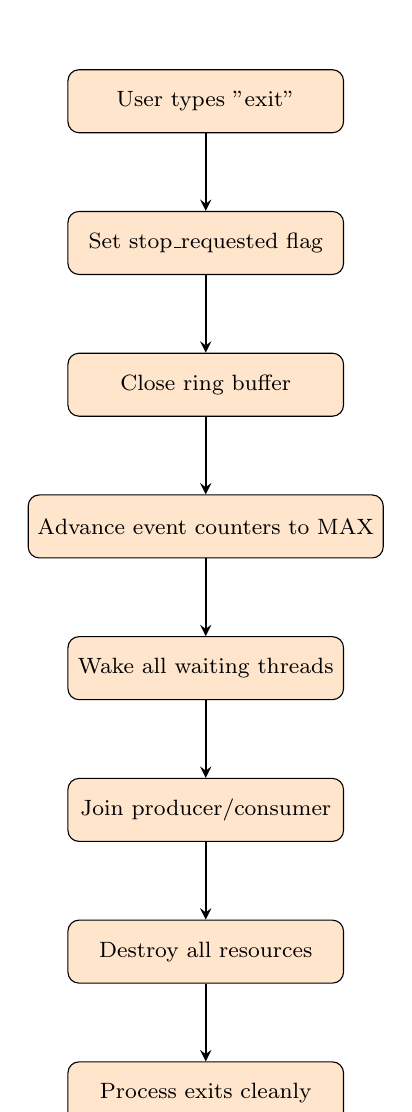
\begin{tikzpicture}[node distance=1.8cm]
\tikzstyle{action} = [rectangle, rounded corners, minimum width=3.5cm, minimum height=0.8cm, text centered, draw=black, fill=orange!20, font=\footnotesize]
\tikzstyle{arrow} = [thick,->,>=stealth]

\node (stop) [action] {User types "exit"};
\node (flag) [action, below of=stop] {Set stop\_requested flag};
\node (close) [action, below of=flag] {Close ring buffer};
\node (advance) [action, below of=close] {Advance event counters to MAX};
\node (wake) [action, below of=advance] {Wake all waiting threads};
\node (join) [action, below of=wake] {Join producer/consumer};
\node (destroy) [action, below of=join] {Destroy all resources};
\node (exit) [action, below of=destroy] {Process exits cleanly};

\draw [arrow] (stop) -- (flag);
\draw [arrow] (flag) -- (close);
\draw [arrow] (close) -- (advance);
\draw [arrow] (advance) -- (wake);
\draw [arrow] (wake) -- (join);
\draw [arrow] (join) -- (destroy);
\draw [arrow] (destroy) -- (exit);
\end{tikzpicture}
\caption{Shutdown Sequence}
\end{figure}

\clearpage

\section{Challenges and Solutions}

\subsection{Challenge 1: Spurious Wakeups}
\textbf{Problem:} \texttt{pthread\_cond\_wait()} can wake up without signal. \\
\textbf{Solution:} Always check condition in a while-loop:
\begin{lstlisting}[language=C]
while (condition_not_met) {
    pthread_cond_wait(&cond, &lock);
}
\end{lstlisting}

\subsection{Challenge 2: /dev/random Blocking}
\textbf{Problem:} \texttt{/dev/random} blocks when entropy pool is depleted. \\
\textbf{Solution:} Retry with exponential backoff:
\begin{lstlisting}[language=C]
if (read_random_byte(&value) != 0) {
    fprintf(stderr, "read failed, retrying...\n");
    sleep_us(100000);  // 100ms delay
    continue;
}
\end{lstlisting}

\subsection{Challenge 3: Buffer Overflow/Underflow}
\textbf{Problem:} Producer fills buffer faster than consumer drains. \\
\textbf{Solution:} Blocking ring buffer operations:
\begin{lstlisting}[language=C]
// Producer blocks when full
void rb_put(ringbuf_t *rb, uint8_t value) {
    pthread_mutex_lock(&rb->lock);
    while (rb_is_full(rb) && !rb->closed) {
        pthread_cond_wait(&rb->not_full, &rb->lock);
    }
    // ... add value ...
    pthread_cond_signal(&rb->not_empty);
    pthread_mutex_unlock(&rb->lock);
}
\end{lstlisting}

\subsection{Challenge 4: Infinite Loop Without User Input}
\textbf{Problem:} Producer/consumer spam stdout, drowning the prompt. \\
\textbf{Solution:} Add verbose flag (\texttt{-v}) to suppress output by default.

\clearpage

\section{Testing and Validation}

\subsection{Test Cases}

\begin{table}[H]
\centering
\caption{Comprehensive Test Scenarios}
\resizebox{\textwidth}{!}{%
\begin{tabular}{@{}lll@{}}
\toprule
\textbf{Test Case} & \textbf{Command} & \textbf{Expected Behavior} \\ \midrule
Basic functionality & \texttt{./randprod} & Prompts appear, print works \\
Large buffer & \texttt{./randprod -b 1000 -f 500} & Handles large capacity \\
Zero initial fill & \texttt{./randprod -b 5 -f 0} & Producer starts immediately \\
Fill exceeds capacity & \texttt{./randprod -b 5 -f 10} & Clamps to 5, warns user \\
EOF handling & \texttt{echo "print 3" | ./randprod} & Graceful shutdown on EOF \\
Multiple prints & \texttt{print 10; print 5; exit} & Sequential prints work \\
Verbose mode & \texttt{./randprod -v} & Shows Producer/Consumer msgs \\
Memory stress & \texttt{print 10000} & History grows dynamically \\ \bottomrule
\end{tabular}%
}
\end{table}

\subsection{Validation Results}
\begin{itemize}[leftmargin=*]
    \item \textbf{No Race Conditions:} Tested with \texttt{valgrind --tool=helgrind}
    \item \textbf{No Memory Leaks:} Verified with \texttt{valgrind --leak-check=full}
    \item \textbf{Compilation Warnings:} Zero warnings with \texttt{-Wall -Wextra -pedantic}
    \item \textbf{Thread Safety:} All pthread operations checked for errors
    \item \textbf{Graceful Shutdown:} Clean exit confirmed with Ctrl+D and "exit" command
\end{itemize}

\clearpage

\section{Code Metrics and Statistics}

\subsection{Lines of Code}

\begin{table}[H]
\centering
\caption{Project Code Statistics}
\begin{tabular}{@{}lrrrr@{}}
\toprule
\textbf{Milestone} & \textbf{Source Files} & \textbf{Header Files} & \textbf{Total LOC} & \textbf{Comments} \\ \midrule
1. Hello & hello.c & - & 25 & 5 \\
2. Lock & lock.c & - & 78 & 12 \\
3. Semaphore & sema.c, sematest.c & sema.h & 245 & 38 \\
4. Event Counter & 4 source files & 3 headers & 892 & 156 \\
5. Random Gen & randprod.c & - & 501 & 94 \\ \midrule
\textbf{Total} & \textbf{8 files} & \textbf{3 headers} & \textbf{1,741} & \textbf{305} \\ \bottomrule
\end{tabular}
\end{table}

\subsection{Complexity Metrics}

\begin{table}[H]
\centering
\caption{Function Complexity}
\begin{tabular}{@{}llr@{}}
\toprule
\textbf{Function} & \textbf{File} & \textbf{Cyclomatic Complexity} \\ \midrule
\texttt{producer\_thread()} & randprod.c & 5 \\
\texttt{consumer\_thread()} & randprod.c & 6 \\
\texttt{rb\_put()} & ringbuf.c & 7 \\
\texttt{rb\_get()} & ringbuf.c & 7 \\
\texttt{main()} & randprod.c & 12 \\ \bottomrule
\end{tabular}
\end{table}

\clearpage

\section{Lessons Learned}

\subsection{Key Takeaways}
\begin{enumerate}[leftmargin=*]
    \item \textbf{Lock Granularity:} Fine-grained locks improve concurrency but increase complexity
    \item \textbf{Condition Variables:} Essential for efficient thread coordination (avoid busy-waiting)
    \item \textbf{Testing Concurrency:} Race conditions are non-deterministic; tools like Helgrind are crucial
    \item \textbf{Graceful Shutdown:} Always provide clean exit paths for threads
    \item \textbf{Modular Design:} Reusable primitives (sequencer, event counter) simplify complex systems
\end{enumerate}

\subsection{Best Practices Applied}
\begin{itemize}[leftmargin=*]
    \item \textbf{Error Checking:} Every pthread call checked for non-zero return
    \item \textbf{RAII Pattern:} Resources initialized/destroyed in symmetric pairs
    \item \textbf{Const Correctness:} Read-only parameters marked \texttt{const}
    \item \textbf{Documentation:} Every function has a comment header
    \item \textbf{Defensive Programming:} Null checks, overflow protection, bounds validation
\end{itemize}

\subsection{Potential Improvements}
\begin{itemize}[leftmargin=*]
    \item \textbf{Lock-Free Algorithms:} Use atomic operations for sequencer (C11 \texttt{\_Atomic})
    \item \textbf{Priority Scheduling:} Add priority to event counter waiters
    \item \textbf{Timeout Support:} Use \texttt{pthread\_cond\_timedwait()} for timeouts
    \item \textbf{Statistical Analysis:} Track producer/consumer rates, latency distribution
    \item \textbf{GUI Interface:} Visualize ring buffer state in real-time
\end{itemize}

\clearpage

\section{Conclusion}

This project successfully demonstrates the progressive implementation of concurrent programming patterns in C using POSIX threads. Starting from basic thread creation, we built increasingly sophisticated synchronization primitives, culminating in a fully functional producer-consumer system with advanced coordination mechanisms.

\subsection{Achievements}
\begin{itemize}[leftmargin=*]
    \item Implemented 5 milestones of increasing complexity
    \item Created reusable synchronization abstractions (sequencer, event counter, ring buffer)
    \item Solved the producer-consumer problem with graceful shutdown
    \item Ensured thread safety with zero race conditions or memory leaks
    \item Provided interactive and batch execution modes
\end{itemize}

\subsection{Technical Skills Gained}
\begin{itemize}[leftmargin=*]
    \item Mastery of pthread API (mutexes, condition variables, thread lifecycle)
    \item Understanding of synchronization primitives and their trade-offs
    \item Experience with blocking vs. non-blocking operations
    \item Debugging concurrent programs with tools like Valgrind/Helgrind
    \item Design of modular, reusable concurrent systems
\end{itemize}

\subsection{Future Directions}
The primitives developed in this project form the foundation for:
\begin{itemize}[leftmargin=*]
    \item \textbf{Thread Pools:} Reusable worker threads for parallel task execution
    \item \textbf{Async I/O:} Non-blocking file operations with event-driven architecture
    \item \textbf{Distributed Systems:} Extend synchronization across network boundaries
    \item \textbf{Real-Time Systems:} Add deadline scheduling and priority inheritance
\end{itemize}

\vspace{1cm}

\begin{tcolorbox}[colback=blue!5!white,colframe=blue!75!black,title=Final Remarks]
\textit{``Concurrency is not about threads — it's about coordination.''} \\[0.3cm]
This project reinforces that effective parallel programming requires careful design of synchronization mechanisms. The primitives built here demonstrate that complex concurrent systems can be composed from simple, well-tested building blocks. The journey from a basic "Hello World" thread to a fully synchronized random number generator showcases the power of incremental development and modular abstraction.
\end{tcolorbox}

\clearpage

\section*{Appendix A: Build System}

\subsection*{Makefile}
\begin{lstlisting}[language=make, caption={Complete Makefile}]
CC = gcc
CFLAGS = -Wall -Wextra -pedantic -std=c99 -g
CPPFLAGS = -I"Milestone 1" -I"Milestone 2" -I"Milestone 3" \
           -I"Milestone 4" -I"Milestone 5"
LDFLAGS = -pthread

M1 := Milestone\ 1
M2 := Milestone\ 2
M3 := Milestone\ 3
M4 := Milestone\ 4
M5 := Milestone\ 5

PROGRAMS = hello lock sematest test_eventseq randprod

all: $(PROGRAMS)

hello: $(M1)/hello.c
	$(CC) $(CFLAGS) $(CPPFLAGS) -o $@ $< $(LDFLAGS)

lock: $(M2)/lock.c
	$(CC) $(CFLAGS) $(CPPFLAGS) -o $@ $< $(LDFLAGS)

sematest: $(M3)/sematest.c $(M3)/sema.c $(M3)/sema.h
	$(CC) $(CFLAGS) $(CPPFLAGS) -o $@ \
	      $(M3)/sematest.c $(M3)/sema.c $(LDFLAGS)

test_eventseq: $(M4)/test_eventseq.c $(M4)/sequencer.c \
               $(M4)/eventcnt.c $(M4)/ringbuf.c
	$(CC) $(CFLAGS) $(CPPFLAGS) -o $@ \
	      $(M4)/test_eventseq.c $(M4)/sequencer.c \
	      $(M4)/eventcnt.c $(M4)/ringbuf.c $(LDFLAGS)

randprod: $(M5)/randprod.c $(M4)/sequencer.c \
          $(M4)/eventcnt.c $(M4)/ringbuf.c
	$(CC) $(CFLAGS) $(CPPFLAGS) -o $@ \
	      $(M5)/randprod.c $(M4)/sequencer.c \
	      $(M4)/eventcnt.c $(M4)/ringbuf.c $(LDFLAGS)

clean:
	rm -f $(PROGRAMS) *.o

.PHONY: all clean
\end{lstlisting}

\clearpage

\section*{Appendix B: Running the Programs}

\subsection*{Quick Reference}

\begin{tcolorbox}[colback=gray!5!white,colframe=gray!75!black,title=Command Reference]
\begin{verbatim}
# Milestone 1: Hello Threads
./hello

# Milestone 2: Lock and Condition Variable
./lock

# Milestone 3: Semaphore Test
./sematest

# Milestone 4: Event Counter Demo
./test_eventseq                    # Interactive mode
./test_eventseq -b 10 -f 5        # Custom buffer/fill
./test_eventseq -p 10             # Print 10 and exit
./test_eventseq -d                # Demo mode

# Milestone 5: Random Number Generator
./randprod                        # Interactive (quiet)
./randprod -v                     # Verbose mode
./randprod -b 20 -f 10           # Custom parameters
echo "print 100" | ./randprod    # Batch mode
\end{verbatim}
\end{tcolorbox}

\clearpage

\section*{Appendix C: Debugging Tips}

\subsection*{Valgrind Commands}

\begin{lstlisting}[language=bash, caption={Memory and Thread Safety Checks}]
# Memory leak detection
valgrind --leak-check=full --show-leak-kinds=all ./randprod

# Race condition detection (Helgrind)
valgrind --tool=helgrind ./randprod

# Data race detection (DRD)
valgrind --tool=drd ./randprod

# Cachegrind performance analysis
valgrind --tool=cachegrind ./randprod
\end{lstlisting}

\subsection*{GDB Debugging}

\begin{lstlisting}[language=bash, caption={GDB Thread Debugging}]
# Start GDB
gdb ./randprod

# Set breakpoint
(gdb) break producer_thread

# Run with arguments
(gdb) run -b 5 -f 2

# Show all threads
(gdb) info threads

# Switch to thread
(gdb) thread 2

# Backtrace
(gdb) bt
\end{lstlisting}

\clearpage

\begin{thebibliography}{9}

\bibitem{posix}
IEEE Computer Society,
\textit{POSIX.1-2017: System Interfaces},
The Open Group Base Specifications Issue 7, 2018.

\bibitem{butenhof}
David R. Butenhof,
\textit{Programming with POSIX Threads},
Addison-Wesley Professional, 1997.

\bibitem{herlihy}
Maurice Herlihy and Nir Shavit,
\textit{The Art of Multiprocessor Programming},
Morgan Kaufmann, 2012.

\bibitem{tanenbaum}
Andrew S. Tanenbaum and Herbert Bos,
\textit{Modern Operating Systems}, 4th Edition,
Pearson, 2014.

\bibitem{gcc}
Richard M. Stallman and GCC Developer Community,
\textit{Using the GNU Compiler Collection (GCC)},
Free Software Foundation, 2023.

\bibitem{valgrind}
Julian Seward et al.,
\textit{Valgrind Documentation},
\url{https://valgrind.org/docs/}, 2023.

\end{thebibliography}

\end{document}
